\subsection*{Solutions}

\begin{solution}[Exercise \ref{exc:which_of_the_following_represent_a_set}]
	\label{sol:which_of_the_following_represent_a_set}$ $

	\begin{enumerate}
		\label{enum:sets_and_numbers_example_solution}

		\item This represents a set since it's well defined. We all know what it
		      means to be registered for a class.
		\item This does not represent a set since it's not well defined. There are
		      many different interpretations of what it means to be a good student
		      (get an \textbf{A} or pass the class or attend class or avoid falling
		      asleep in class or don't cause trouble in class)
	\end{enumerate}
\end{solution}

\begin{solution}[Exercise \ref{exc:simplify_the_following_expressions}]
	\label{sol:simplify_the_following_expressions}$ $

	\begin{itemize}
		\label{item:simplify_the_following_expressions_solutions}

		\item $(-4, \infty) \cup [-8, 3] = [-8, \infty)$
		\item $(-4, \infty) \cup (-\infty, 2] = (-\infty, \infty) = \mathbb{R}$
		\item $(-4, \infty) \cap (-\infty, 2] = (-4, 2]$
		\item $(-4, \infty) \cap [-10, -5] = \emptyset$
	\end{itemize}
\end{solution}

\begin{solution}[Exercise
		\ref{exc:convert_8_radians_into_degrees_and_8_into_radians}]
	\label{sol:convert_8_radians_into_degrees_and_8_into_radians}

	Since $2\pi = 360^{\circ} \qquad \frac{2\pi}{360^{\circ}} = 1 = \frac{360^{\circ}}{2\pi}$.
	We're trying to cancel out the radians. So, to do this, we will need to have
	the radians on the bottom, and the degrees on the top. After we do the
	multiplication, we will be left with the degrees.

	\begin{align*}
		8\rad \times \left(\frac{360^{\circ}}{2\pi \rad}\right) & =
		\frac{8 \times 360^{\circ}}{2\pi}                                                    \\
		                                                        & = \frac{1440^{\circ}}{\pi} \\
		                                                        & \approx 458.4
		.\end{align*}

	Now, let's convert $8^{\circ}$ into $8$ radians.

	\begin{align*}
		8^{\circ} \left(\frac{\pi \rad}{180^{\circ}}\right) & =
		\frac{8\pi}{180} \rad                                                       \\
		                                                    & = \frac{\pi}{45} \rad \\
		.\end{align*}
\end{solution}

\begin{solution}[Exercise
		\ref{exc:what_is_the_arc_length_spanned_by_a_40_degree_angle_on_a_circle_of_radius_30_meters}]
	\label{sol:what_is_the_arc_length_spanned_by_a_40_degree_angle_on_a_circle_of_radius_30_meters}

	Convert $40^{\circ}$ into radians:

	\begin{align*}
		40^{\circ} \times \left(\frac{\pi}{180^{\circ}}\right) & =
		\frac{40\pi}{180} \rad                                                     \\
		                                                       & = \frac{4\pi}{18} \\
		                                                       & = \frac{2\pi}{9}  \\
		                                                       & \approx 0.7       \\
		.\end{align*}

	Now we're ready to compute the arc length:

	\begin{align*}
		s & = r \times \mid \theta \mid     \\
		  & = (30m) \times (\frac{2\pi}{9}) \\
		  & = \frac{20\pi}{3}m
		.\end{align*}
\end{solution}

\begin{solution}[Exercise \ref{exc:period}]
	\label{sol:period}

	The \textbf{period} for the graph is $2$. The reason is because if you shift
	the graph $2$ units either left or right, you will get the same graph.

	Another way to find the period is the take an $x$-intercept and the
	$x$-intercept to the right of it and subtract the two: $10 - 8 = 2$
\end{solution}

\begin{solution}[Exercise \ref{exc:midline_and_amplitude}]
	\label{sol:midline_and_amplitude}

	The \textbf{midline} of the graph is $0$.
	\[ \frac{1 + (-1)}{2} = \frac{0}{2} = 0 \].

	The \textbf{amplitude} of the graph is $1$, which is the distance from the
	maximum or minimum to the midline.
\end{solution}

\begin{solution}[Exercise \ref{exc:angle_of_theta}]
	\label{sol:angle_of_theta}

	\begin{align*}
		P & = (\cos(\theta), \sin(\theta)) \\
		  & = \cos(\theta) = -\frac{3}{5}  \\
		  & = \sin(\theta) = \frac{4}{5}
		.\end{align*}
\end{solution}

\begin{solution}[Exercise \ref{exc:using_r_cos_and_r_sin}]
	\label{sol:using_r_cos_and_r_sin}

	The point $Q$ is specified by $\alpha$ on the circumference of a circle of
	radius $6$ units. Thus \ldots

	\[ Q = (6 \cos (\alpha), 6 \sin (\alpha)) \].
\end{solution}

\begin{solution}[Exercise \ref{exc:find_cos}]
	\label{sol:find_cos}

	Since the Pythagorean Identity gives us an equation involving sin and cos, we
	can use it to find one of the values when we know the other value. In this
	case, we know the value of $\sin (A)$, so we can use the Pythagorean Identity
	to find $\cos (A)$ :

	\begin{align*}
		 & \qquad\sin^{2} (A) + \cos^{2} (A) = 1                    \\
		 & \implies \left(\frac{1}{2}\right)^{2} + \cos^{2} (A) = 1 \\
		 & \implies \cos^{2} (A) = 1 - \left(\frac{1}{3}\right)^{2} \\
		 & \implies \cos (A) = - \sqrt{\frac{8}{9}}                 \\
		 & \implies \cos (A) = -\frac{2\sqrt{2}}{3}
		.\end{align*}

	The reason I made the answer negative is because the value of cos in Quadrant
	II is negative. If cos was in Quadrant I, then the answer would be positive.
\end{solution}

\begin{solution}[Exercise \ref{exc:find_tan_sec_csc_cot_1}]
	\label{sol:find_tan_sec_csc_cot_1}

	\begin{align*}
		\tan \left(\frac{\pi}{6}\right) & = \frac{\sin \left(\frac{\pi}{6}\right)}{\cos \left(\frac{\pi}{6}\right)} \\
		                                & = \frac{\frac{1}{2}}{\frac{\sqrt{3}}{2}}                                  \\
		                                & = \frac{1}{\sqrt{3}} = \frac{\sqrt{3}}{3}                                 \\
		\sec \left(\frac{\pi}{6}\right) & = \frac{1}{\cos \left(\frac{\pi}{6}\right)}                               \\
		                                & = \frac{1}{\frac{\sqrt{3}}{2}}                                            \\
		                                & = \frac{2}{\sqrt{3}} = \frac{2\sqrt{3}}{3}                                \\
		\csc \left(\frac{\pi}{6}\right) & = \frac{1}{\sin \left(\frac{\pi}{6}\right)}                               \\
		                                & = \frac{1}{\frac{1}{2}}                                                   \\
		                                & = 2                                                                       \\
		\cot \left(\frac{\pi}{6}\right) & = \frac{\cos \left(\frac{\pi}{6}\right)}{\sin \left(\frac{\pi}{6}\right)} \\
		                                & = \frac{\frac{\sqrt{3}}{2}}{\frac{1}{2}}                                  \\
		                                & = \sqrt{3}                                                                \\
		.\end{align*}
\end{solution}

\begin{solution}[Exercise \ref{exc:find_tan_sec_csc_cot_2}]
	\label{sol:find_tan_sec_csc_cot_2}

	\begin{align*}
		\tan \left(\frac{\pi}{4}\right) & = \frac{\sin \left(\frac{\pi}{4}\right)}{\cos \left(\frac{\pi}{4}\right)} \\
		                                & = \frac{\frac{\sqrt{2}}{2}}{\frac{\sqrt{2}}{2}}                           \\
		                                & = 1                                                                       \\
		\sec \left(\frac{\pi}{4}\right) & = \frac{1}{\cos \left(\frac{\pi}{4}\right)}                               \\
		                                & = \frac{1}{\frac{\sqrt{2}}{2}}                                            \\
		                                & = \frac{2}{\sqrt{2}} = \sqrt{2}                                           \\
		\csc \left(\frac{\pi}{4}\right) & = \frac{1}{\sin \left(\frac{\pi}{4}\right)}                               \\
		                                & = \frac{1}{\frac{\sqrt{2}}{2}}                                            \\
		                                & = \frac{2}{\sqrt{2}} = \sqrt{2}                                           \\
		\cot \left(\frac{\pi}{4}\right) & = \frac{\cos \left(\frac{\pi}{4}\right)}{\sin \left(\frac{\pi}{4}\right)} \\
		                                & = \frac{\frac{\sqrt{2}}{2}}{\frac{\sqrt{2}}{2}}                           \\
		                                & = 1                                                                       \\
		.\end{align*}
\end{solution}

\begin{solution}[Exercise \ref{exc:find_tan_sec_csc_cot_3}]
	\label{sol:find_tan_sec_csc_cot_3}

	\begin{align*}
		\tan \left(\frac{\pi}{3}\right) & = \frac{\sin \left(\frac{\pi}{3}\right)}{\cos \left(\frac{\pi}{3}\right)} \\
		                                & = \frac{\frac{\sqrt{3}}{2}}{\frac{1}{2}}                                  \\
		                                & = \sqrt{3}                                                                \\
		\sec \left(\frac{\pi}{3}\right) & = \frac{1}{\cos \left(\frac{\pi}{3}\right)}                               \\
		                                & = \frac{1}{\frac{1}{2}}                                                   \\
		                                & = 2                                                                       \\
		\csc \left(\frac{\pi}{3}\right) & = \frac{1}{\sin \left(\frac{\pi}{3}\right)}                               \\
		                                & = \frac{1}{\frac{\sqrt{3}}{2}}                                            \\
		                                & = \frac{2}{\sqrt{3}} = \frac{2\sqrt{3}}{3}                                \\
		.\end{align*}
\end{solution}

\begin{solution}[Exercise \ref{exc:find_reference_angle_1}]
	\label{sol:find_reference_angle_1}

	The reference angle for $150^{\circ}$ is $30^{\circ}$. \\
	The reference angle for $\frac{5\pi}{4}$ is $\frac{\pi}{4}$.
\end{solution}

\begin{solution}[Exercise \ref{exc:transform_the_graph_of_f_to_g}]
	\label{sol:transform_the_graph_of_f_to_g}

	It should be clear that function $g$ is a sinusoidal function of the form
	$y = A\sin(\omega(t - h)) + k$ where $A = 2, \omega = 1, h = 0, k = -3$.

	After inspecting the rules for the functions $f$ and $g$, we should notice
	that we could construct the function $g(t) = 2\sin(t) - 3$ by multiplying the
	outputs of the function $f(t) = \sin(t)$ by $2$ and then subtracting $3$ from
	the result. We can express this algebraically with the equation below:
	\[ g(t) = 2 f(t) - 3 \].

	Based on what we know about the graph transformations, we can conclude that we
	can obtain graph of $g$ by starting with the graph of $f$ and first stretching
	it vertically by a factor of $2$ and then shifting it down $3$ units. Since
	$f(t) = \sin(t)$ has amplitude of $1$ unit, if we stretch it vertically by a
	factor of $2$, then we'll double the amplitude, so we should expect that the
	amplitude of $g$ to be $2$ units. Also, since $f(t) = \sin(t)$ has midline $y
		= 0$, when we shift it down $3$ units, the resulting midline for the function
	$g$ will be $y = -3$.

	\begin{center}
		\textbf{period:} $2\pi$ units \\
		\textbf{midline:} $y = -3$ \\
		\textbf{amplitude:} $2$ units \\
		\textbf{horizontal shift:} $0$ units
	\end{center}

	\begin{figure}[H]
		\centering

		\begin{tikzpicture}
			\begin{axis}[
					my axis style,
					width=\textwidth,
					height=.5\textwidth,
				]
				\addplot[
					domain=-10:10,
					red,
					thick,
					<->
				]
				{sin(deg(x))};
				\addplot[
					domain=-10:10,
					blue,
					thick,
					<->
				]
				{2*sin(deg(x))-3};
			\end{axis}
		\end{tikzpicture}

		\caption{The graph of {\color{red}$f(t) = \sin(t)$} and {\color{blue}$g(t) = 2\sin(t) - 3$}}
		\label{fig:the_graph_of_y_cos_theta_and_y_sin_theta_1}
	\end{figure}
\end{solution}

\begin{solution}[Exercise
		\ref{exc:find_two_algebraic_rules_for_the_function_y_g_t}]
	\label{sol:find_two_algebraic_rules_for_the_function_y_g_t}

	Let's start by finding the values of $A, \omega, k$. To do this, we need to
	find the midline, amplitude, and period.

	The midline is $y = -3$, which dictates what the value of $k$ is. \\
	The amplitude is the distance from the maximum/minimum to the midline. The
	amplitude is $4$ units. \\
	The period is the distance from each maximum/minimum. $6.5 - 0.5 = 6$ units.
	The period doesn't actually appear as a number in the algebraic rule for the
	function. But the period is connected with the value that we use of $\omega$.
	$\omega$ causes a horizontal stretch which gives us the desired period.
	\[
		6 = 2\pi \times \frac{1}{\omega} = \frac{2\pi}{6} = \boxed{\frac{\pi}{3}}
	\].
	When we're trying to find a formula that involves sin, we want to think in
	terms of sin waves, which start at the midline and come up out of the midline.
	So, we'll want to find a place in this function where the function is crossing
	through the midline and coming up out of the midline. That would be at the
	point: $(0, -1)$. So, for the sin function, $h = -1$. For cos, it's the
	opposite. Cos starts at the maximum, and goes down to the midline. That would
	be at the point: $(0, 0.5)$. So, for the cos function, $h = 0.5$.
	\[
		g(t) = 4\sin \left(\frac{\pi}{3} \left(t + 1\right)\right) - 3 \qquad
		g(t) = 4\cos \left(\frac{\pi}{3} \left(t - \frac{1}{2}\right)\right) - 3
	\].
\end{solution}

\begin{solution}[Exercise \ref{exc:evaluate_invs_sin}]
	\label{sol:evaluate_invs_sin}$ $

	\begin{itemize}
		\item To evaluate $\sin^{-1} (-\frac{1}{2})$, we need to find a value, $p$,
		      such that $-\frac{\pi}{2} \le p \le \frac{\pi}{2}$ and $\sin (p) =
			      -\frac{1}{2}$. $p = -\frac{\pi}{6}$. Thus, $\sin^{-1} (-\frac{1}{2}) =
			      -\frac{\pi}{6}$.
		\item To evaluate $\sin (\sin^{-1} (\frac{\sqrt{3}}{2}))$, we need to first
		      find $\sin^{-1} (\frac{\sqrt{3}}{2})$, such that $-\frac{\pi}{2} \le p
			      \le \frac{\pi}{2}$. $p = \frac{\pi}{3}$. Thus, $\sin^{-1}
			      (\frac{\sqrt{3}}{2}) = \frac{\pi}{3}$. Now we can evaluate that:
		      \[
			      \sin \left(\sin^{-1} \left(\frac{\sqrt{3}}{2}\right)\right) = \sin
			      \left(\left(\frac{\pi}{3}\right)\right) = \frac{\sqrt{3}}{2}
		      \].
	\end{itemize}
\end{solution}

\begin{solution}[Exercise \ref{exc:evaluate_invs_cos}]
	\label{sol:evaluate_invs_cos}$ $

	\begin{itemize}
		\item To evaluate $\cos^{-1} (0)$, we need to find a value, $p$, such that
		      $0 \le p \le \pi$ and $\cos (p) = 0$. $p = \frac{\pi}{2}$. Thus,
		      $\cos^{-1} (0) = \frac{\pi}{2}$.
		\item To evaluate $\cos (\cos^{-1} (\frac{1}{2}))$, we need to first find
		      $\cos^{-1} (\frac{1}{2})$, such that $0 \le p \le \pi$. $p =
			      \frac{\pi}{3}$. Thus, $\cos^{-1} (\frac{1}{2}) = \frac{\pi}{3}$. Now we
		      can evaluate that:
		      \[
			      \cos \left(\cos^{-1} \left(\frac{1}{2}\right)\right) = \cos
			      \left(\frac{\pi}{3}\right) = -\sqrt{3}
		      \].
	\end{itemize}
\end{solution}

\begin{solution}[Exercise \ref{exc:evaluate_invs_tan}]
	\label{sol:evaluate_invs_tan}$ $
	\begin{itemize}
		\item To evaluate $\tan^{-1} (1)$, we need to find a value, $p$, such that
		      $-\frac{\pi}{2} \le p \le \frac{\pi}{2}$ and $\tan (p) = 1$. $p =
			      \frac{\pi}{4}$. Thus, $\tan^{-1} (1) = \frac{\pi}{4}$.
		\item To evaluate $\tan (\tan^{-1} (-\sqrt{3}))$, we need to first find
		      $\tan^{-1} (-\sqrt{3})$, such that $-\frac{\pi}{2} \le p \le
			      \frac{\pi}{2}$. $p = -\frac{\pi}{3}$. Thus, $\tan^{-1} (-\sqrt{3}) =
			      -\frac{\pi}{3}$. Now we can evaluate that:
		      \[
			      \tan \left(\tan^{-1} \left(-\sqrt{3}\right)\right) = \tan
			      \left(-\frac{\pi}{3}\right) = -\sqrt{3}
		      \].
	\end{itemize}

\end{solution}

\begin{solution}[Exercise \ref{exc:inv_sin_2}]
	\label{sol:inv_sin_2}

	The sin value $-0.555$ isn't a "friendly" sin value. We don't know what input
	for the sin function is related to the output $-0.555$, so we need to utilize
	the inverse sin function in order to solve the equation:

	\begin{equation*}
		\begin{alignedat}{3}
			&\qquad\sin (t) &&= -0.555 \\
			&\implies \sin^{-1} (\sin (t)) &&= \sin^{-1} (-0.555) \\
			&\implies \qquad\qquad t &&= \sin^{-1} (-0.555) \approx -0.588
		\end{alignedat}
		.\end{equation*}

	Although we've found one solution to the equation, we aren't done yet! The
	inverse sin inverse only gives us one value, but we know that the periodic
	nature of the sin function suggests that there are infinitely many solutions
	to an equation like this.

	We can find all of the solutions by using the solution that we found using the
	inverse sin function along with the fact that the sin function has period
	$2\pi$. Since the sin function has a period of $2\pi$ units, we know that the
	outputs repeat every $2\pi$ units. So if $t \approx -0.588$ is a solution, the
	values represented by $t \approx -0.55 + 2k\pi, k \in \mathbb{Z}$. That gives
	us more solutions, but we're still missing half of the solutions. Since
	$\sin(t) = (\pi - t)$, we can use this identity to find our other half missing
	solution. $t = \pi - (-0.588) + 2k\pi, k \in \mathbb{Z}$. Therefore, the
	complete solution to the equation is:
	\[
		t \approx -0.588 + 2k\pi \textrm{ or } t \approx \pi + 0.588 + 2k\pi
		\textrm{ for all } k \in \mathbb{Z}
	\].
\end{solution}

\begin{solution}[Exercise
		\ref{exc:find_value_for_all_six_trigonometric_functions}]
	\label{sol:find_value_for_all_six_trigonometric_functions}

	To find the value for all the $6$ trig functions for the angle $\alpha$, we
	need to find the value for the hypotenuse. For this, we can use the
	Pythagorean Theorem:
	\begin{align*}
		\qquad         & a^{2} + b^{2} = c^{2}     \\
		\implies\qquad & 12^{2} + 9^{2} = c^{2}    \\
		\implies\qquad & 144 + 81 = c^{2}          \\
		\implies\qquad & 225 = c^{2}               \\
		\implies\qquad & \sqrt{225} = \sqrt{c^{2}} \\
		\implies\qquad & c = 15                    \\
		.\end{align*}

	Now we can use \textbf{SOH CAH TOA} to find the value for all $6$ trig
	functions.
	\begin{align*}
		\sin (\alpha) = \frac{\textrm{OPP}}{\textrm{HYP}}
		\implies \sin (\alpha) = \frac{9}{15} = \frac{3}{5}          \\
		\cos (\alpha) = \frac{\textrm{ADJ}}{\textrm{HYP}}
		\implies \cos (\alpha) = \frac{12}{15} = \frac{4}{5}         \\
		\tan (\alpha) = \frac{\textrm{OPP}}{\textrm{ADJ}}
		\implies \tan (\alpha) = \frac{9}{12} = \frac{3}{4}          \\
		\sec (\alpha) = \frac{1}{\cos (\alpha)}
		\implies \sec (\alpha) = \frac{1}{\frac{4}{5}} = \frac{5}{4} \\
		\csc (\alpha) = \frac{1}{\sin (\alpha)}
		\implies \csc (\alpha) = \frac{1}{\frac{3}{5}} = \frac{5}{3} \\
		\cot (\alpha) = \frac{1}{\tan (\alpha)}
		\implies \cot (\alpha) = \frac{1}{\frac{3}{4}} = \frac{4}{3} \\
		.\end{align*}
\end{solution}

\begin{solution}[Exercise \ref{exc:solving_a_right_triangle}]
	\label{sol:solving_a_right_triangle}

	We know that we have an angle with a $90^{\circ}$ and a $60^{\circ}$, which
	implies that $A = 30^{\circ}$.

	We need to create an equation with only either $b$ or $c$ as the unknown:
	\begin{align*}
		\qquad         & \sin (30^{\circ}) = \frac{7}{c} \\
		\implies\qquad & \frac{1}{2} = \frac{7}{c}       \\
		\implies\qquad & c = 14                          \\
		.\end{align*}

	Now we can use the Pythagorean Theorem to solve for $b$ :
	\begin{align*}
		\qquad         & a^{2} + b^{2} = c^{2}     \\
		\implies\qquad & 7^{2} + b^{2} = 14^{2}    \\
		\implies\qquad & 49 + b^{2} = 196          \\
		\implies\qquad & b^{2} = 147               \\
		\implies\qquad & \sqrt{b^{2}} = \sqrt{147} \\
		\implies\qquad & b = 7\sqrt{3}             \\
		.\end{align*}

	\begin{figure}[H]
		\centering

		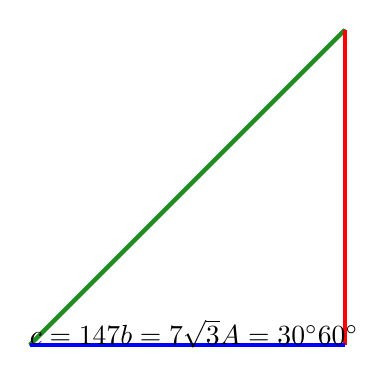
\begin{tikzpicture}
			\coordinate (a) at (0,0);
			\coordinate (b) at (4,0);
			\coordinate (c) at (4,4);

			\draw (a) -- (c) -- (b) -- cycle;

			\draw[ultra thick,ForestGreen] (a) -- (c);
			\draw[ultra thick,red] (c) -- (b);
			\draw[ultra thick,blue] (a) -- (b);

			\tkzLabelSegment (a,c) {$c = 14$};
			\tkzLabelSegment (c,b) {$7$};
			\tkzLabelSegment[below=2pt](a,b){$b = 7\sqrt{3}$};
			\tkzMarkAngle[mark=none](b,a,c);
			\tkzMarkAngle[mark=none](a,c,b);
			\tkzLabelAngle[pos=1.7](b,a,c){$A = 30^{\circ}$};
			\tkzLabelAngle[pos=0.6](a,c,b){$60^{\circ}$};
		\end{tikzpicture}

		\caption{}
		\label{fig:solving_a_right_triangle_2}
	\end{figure}
\end{solution}

\begin{solution}[Exercise \ref{exc:law_of_sines}]
	\label{sol:law_of_sines}

	We can easily find $\theta$ since we know that the sum of the angle-measures
	in a triangle is always $180$. So:
	\[
		\theta + 55^{\circ} + 75^{\circ} = 180^{\circ} \implies \theta = 50^{\circ}
	\].

	Now we can use the \textbf{Law of Sines} to find $m$ and $n$.

	\begin{align*}
		\frac{\sin (\theta)}{m} = \frac{\sin (55^{\circ})}{8} & \implies \frac{m}{\sin (\theta)} = \frac{8}{\sin (55^{\circ})}                        \\
		                                                      & \implies \frac{m}{\sin (50^{\circ})} = \frac{8}{\sin (55^{\circ})}                    \\
		                                                      & \implies \qquad m = \frac{8 \times \sin (50^{\circ})}{\sin (55^{\circ})} \approx 7.48
		.\end{align*}

	and

	\begin{align*}
		\frac{\sin (75^{\circ})}{n} = \frac{\sin (55^{\circ})}{8} & \implies \frac{n}{\sin (75^{\circ})} = \frac{8}{\sin (55^{\circ})}            \\
		                                                          & \implies n = \frac{8 \times \sin (75^{\circ}}{\sin (55^{\circ})} \approx 9.43
		.\end{align*}

	\begin{figure}[H]
		\centering

		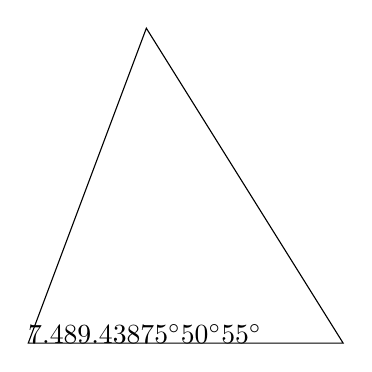
\begin{tikzpicture}
			\coordinate (a) at (0,0);
			\coordinate (b) at (4,0);
			\coordinate (c) at (1.5,4);

			\draw (a) -- (c) -- (b) -- cycle;

			\tkzLabelSegment (a,c) {$7.48$};
			\tkzLabelSegment (c,b) {$9.43$};
			\tkzLabelSegment[below=2pt](a,b){$8$};

			\tkzMarkAngle[mark=none](b,a,c);
			\tkzLabelAngle[pos=0.5](b,a,c){$75^{\circ}$};
			\tkzMarkAngle[mark=none](c,b,a);
			\tkzLabelAngle[pos=0.5](c,b,a){$50^{\circ}$};
			\tkzMarkAngle[mark=none](a,c,b);
			\tkzLabelAngle[pos=0.5](a,c,b){$55^{\circ}$};
		\end{tikzpicture}

		\caption{}
		\label{fig:law_of_sines_with_missing_angles_and_side_lengths_2}
	\end{figure}
\end{solution}

\begin{solution}[Exercise \ref{exc:law_of_cosines}]
	\label{sol:law_of_cosines}

	We can use the \textbf{Law of Cosines} to find $w$.

	\begin{align*}
		\qquad         & w^{2} = 12^{2} + 10^{2} - 2(12)(10) \times \cos(70^{\circ}) \\
		\implies\qquad & w^{2} = 144 + 100 - 240 \times \cos(70^{\circ})             \\
		\implies\qquad & w = \sqrt{144 + 100 - 240 \times \cos(70^{\circ})}          \\
		\implies\qquad & w \approx 12.725
		.\end{align*}

	Now that we know $w$, we now know an angle and the side opposite that angle,
	so we can use the \textbf{Law of Sines} to find either of the other angles.
	Let's find $\beta$.

	\begin{align*}
		\qquad         & \frac{\sin (\beta)}{10} = \frac{\sin (70^{\circ})}{w}                                   \\
		\implies\qquad & \sin (\beta) = \frac{10 \times \sin (70^{\circ})}{w}                                    \\
		\implies\qquad & \sin^{-1} (\sin (\beta)) = \sin^{-1} \left(\frac{10 \times \sin (70^{\circ})}{w}\right) \\
		\implies\qquad & \qquad\beta = \sin^{-1} \left(\frac{10 \times \sin (70^{\circ})}{w}\right)              \\
		\implies\qquad & \qquad\beta \approx 47.6^{\circ}
		.\end{align*}

	Finally, we can find $\alpha$ by using the fact that the sum of the
	angle-measures in a triangle is always $180^{\circ}$.

	\begin{equation*}
		\begin{alignedat}{3}
			\qquad&\alpha + \beta + 70^{\circ} &&= 180^{\circ} \\
			\implies\qquad&\alpha + 47.6^{\circ} + 70^{\circ} &&= 180^{\circ} \\
			\implies\qquad&\alpha + 47.6^{\circ} + 70^{\circ} &&= 180^{\circ} \\
			\implies\qquad&\alpha &&\approx 62.4^{\circ} \\
		\end{alignedat}
		.\end{equation*}

	\begin{figure}[H]
		\centering

		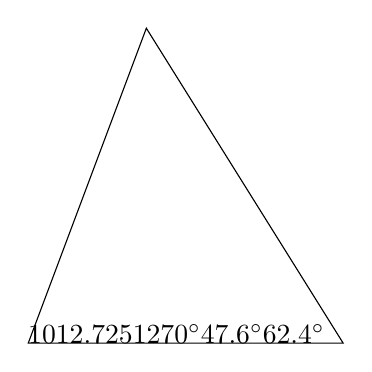
\begin{tikzpicture}
			\coordinate (a) at (0,0);
			\coordinate (b) at (4,0);
			\coordinate (c) at (1.5,4);

			\draw (a) -- (c) -- (b) -- cycle;

			\tkzLabelSegment (a,c) {$10$};
			\tkzLabelSegment (c,b) {$12.725$};
      \tkzLabelSegment[below=2pt](a,b){$12$};

			\tkzMarkAngle[mark=none](b,a,c);
			\tkzLabelAngle[pos=0.5](b,a,c){$70^{\circ}$};
			\tkzMarkAngle[mark=none](c,b,a);
			\tkzLabelAngle[pos=0.5](c,b,a){$47.6^{\circ}$};
			\tkzMarkAngle[mark=none](a,c,b);
			\tkzLabelAngle[pos=0.8](a,c,b){$62.4^{\circ}$};
		\end{tikzpicture}

		\caption{}
		\label{fig:law_of_cosines_2}
	\end{figure}
\end{solution}

\begin{solution}[Exercise \ref{exc:sum_of_angles}]
  \label{sol:sum_of_angles}$ $

  \begin{itemize}
    \item Since $75^{\circ} = 45^{\circ} + 30^{\circ}$, we can use the cos of a
      sum-of-angles identity to calculate $\cos (75^{\circ})$:

      \begin{align*}
        \cos (75^{\circ}) &= \cos(45^{\circ} + 30^{\circ}) \\
                          &= \cos (45^{\circ})\cos (30^{\circ}) - \sin (45^{\circ})\sin (30^{\circ}) \\
                          &= \frac{\sqrt{2}}{2} \times \frac{\sqrt{3}}{2} - \frac{\sqrt{2}}{2} \times \frac{1}{2} \\
                          &= \frac{\sqrt{6}}{4} - \frac{\sqrt{2}}{4} \\
                          &= \frac{\sqrt{6} - \sqrt{2}}{4} \\
      .\end{align*}

    \item Since $-15^{\circ} = 30^{\circ} - 45^{\circ}$, we can use the sin of
      a difference-of-angles identity to calculate $\sin (-15^{\circ})$:

      \begin{align*}
        \sin (-15^{\circ}) &= \sin(30^{\circ} - 45^{\circ}) \\
                           &= \sin (30^{\circ})\cos (45^{\circ}) - \sin (45^{\circ})\cos (30^{\circ}) \\
                           &= \frac{1}{2} \times \frac{\sqrt{2}}{2} - \frac{\sqrt{2}}{2} \times \frac{\sqrt{3}}{2} \\
                           &= \frac{\sqrt{2}}{4} - \frac{\sqrt{6}}{4} \\
                           &= \frac{\sqrt{2} - \sqrt{6}}{4} \\
      .\end{align*}

    \item Since $\frac{11\pi}{12} = \frac{3\pi}{12} + \frac{8\pi}{12} \implies
      \frac{\pi}{4} + \frac{2\pi}{3}$, we can use the sin of a sum-of-angles
      identity to calculate $\sin (\frac{11\pi}{12})$:

      \begin{align*}
        \sin \left(\frac{11\pi}{12}\right) &= \sin \left(\frac{\pi}{4} + \frac{2\pi}{3}\right) \\
                                           &= \sin \left(\frac{\pi}{4}\right)\cos \left(\frac{2\pi}{3}\right) + \sin \left(\frac{2\pi}{3}\right)\cos \left(\frac{\pi}{4}\right) \\
                                           &= \frac{\sqrt{2}}{2} \times \left(-\frac{1}{2}\right) + \frac{\sqrt{3}}{2} \times \frac{\sqrt{2}}{2} \\
                                           &= -\frac{\sqrt{2}}{4} + \frac{\sqrt{6}}{4} \\
                                           &= \frac{-\sqrt{2} + \sqrt{6}}{4} \\
      .\end{align*}
  \end{itemize}
\end{solution}

\begin{solution}[Exercise \ref{exc:sin_alpha_1_over_3_in_quadrant_2}]
  \label{sol:sin_alpha_1_over_3_in_quadrant_2}

  First, let's find $\cos (\alpha)$ since we need this value to use the
  double-angle identity for sin. To find $\cos (\alpha)$, let's use the
  Pythagorean identity:

  \begin{align*}
    \qquad&\sin^{2} (\alpha) + \cos^{2} (\alpha) = 1 \\
    \implies\qquad&\left(\frac{1}{3}\right)^{2} + \cos^{2} (\alpha) = 1 \\
    \implies\qquad&\frac{1}{9} + \cos^{2} (\alpha) = 1 \\
    \implies\qquad&\cos^{2} (\alpha) = 1 - \frac{1}{9} \\
    \implies\qquad&\cos^{2} (\alpha) = \frac{8}{9} \\
    \implies\qquad&\cos^{2} (\alpha) = -\frac{2\sqrt{2}}{3} \\
  .\end{align*}

  Now we can use the double-angle identities to find $\sin (2\alpha)$ and $\cos
  (2\alpha)$. Let's start with $\sin (2\alpha)$:

  \begin{align*}
    \sin (2\alpha) &= 2\sin (\alpha)\cos (\alpha) \\
                   &= 2\left(\frac{1}{3}\right)\left(-\frac{2\sqrt{2}}{3}\right) \\
                   &= -\frac{4\sqrt{2}}{9} \\
  .\end{align*}

  I'm going to use the $\cos (2\alpha) = 1 - 2\sin^{2} (\alpha)$:

  \begin{align*}
    \cos (2\alpha) &= 1 - 2\sin^{2} (\alpha) \\
                   &= 1 - 2\left(\frac{1}{3}\right)^{2} \\
                   &= 1 - 2 \times \frac{1}{9} \\
                   &= 1 - \frac{2}{9} \\
                   &= \frac{7}{9} \\
  .\end{align*}

  Now, we can find $\tan (2\alpha)$:

  \begin{align*}
    \tan (2\alpha) &= \frac{\sin (2\alpha)}{\cos (2\alpha)} \\
                   &= \frac{-\frac{4\sqrt{2}}{9}}{\frac{7}{9}} \\
                   &= -\frac{4\sqrt{2}}{9} \times \frac{9}{7} \\
                   &= -\frac{4\sqrt{2}}{7} \\
  .\end{align*}
\end{solution}

\begin{solution}[Exercise \ref{exc:multiply_vectors_by_scalers}]
  \label{sol:multiply_vectors_by_scalers}
\end{solution}
